\chapter{Hardware Reconfigurable}

\section{FPGAs}

La fabricación de dispositivos semiconductores es un complejo y
costoso proceso a largo plazo. En particular, el costo de fabricación
y la necesidad de llegar sin demoras con el producto al mercado hacen
que no se toleren fallas. Por tal motivo, se torna de gran importancia
las faces de prueba y verificación del diseño antes de la
fabricación. Desafortunadamente, el alto costo y los largos plazos de
diseño dificultan enormemente el prototipado antes de que comience la
producción en grandes volúmenes. Es necesaria una alternativa a la
implementación en chip que permita una verificación y prototipado a
corto plazo de bajo costo. A tal fin, últimas décadas se comenzaron a
construir chips reconfigurables que puedan ser programados para
realizar cualquier función propia de los chip de aplicaciones
especificas. Por ejemplo, la compañía Xilinx, ofreció su primer chip
en 1984, que contiene arreglo de celdas lógicas (LCAs) programables
por el usuario en casi cualquier configuración. Tales dispositivos son
conocidos actualmente como FPGAs por sus siglas en Ingles para
\textit{Field Programmable Gate Array}.

Inicialmente las FPGAs solo podrían ser programadas para cumplir las
funciones de circuitos digitales simples. Sin embargo, con la mejora
de la tecnología~\cite{Etiqueta02} fue posible incrementar capacidad
de las FPGAs hasta el punto en que gran parte de los chips actualmente
fabricados pueden ser completamente programados dentro de las
mismas. Esto último permite realizar el prototipado de dichos chips en
plazos muchos más cortos y a menor costo que los requeridos para la
fabricación del chip en cuestión. Entre las ventajas que ofrecen las
FPGAs se destaca la capacidad de reconfigurar el diseño parcial o
totalmente para su actualización o corrección de errores a un costo
relativamente bajo.

Los diseños implementados en FPGA tienen en general mas área, menos
velocidad y mayor consumo que los implementados en ASIC. Sin embargo,
además de la función de prototipado previamente mencionada, las FPGAs
actuales están siendo cada ves más utilizadas como objetivo final en
el desarrollo de productos. Esto último se debe a que muchos proyectos
no requieren operar en el máximo rendimiento posible dado por la
tecnología. En su lugar, priorizan los tiempos de ejecución más
rápidos y la mayor flexibilidad y capacidad de adaptación que ofrecen
las FPGAs.

Las mencionadas ventajas que ofrecen las FPGAs actuales no se
encontraban presente en las versiones iniciales de las mismas. Fue con
el paso del tiempo que las FPGAs pudieron disminuir su costo y mejorar
la eficiencia en el consumo de energía. Los diseños de FPGAs actuales
poco tienen que ver con los primeras diseños aparecidos en la década
de los 80. Actualmente las FPGAs ofrecen densidades de millones de
puertas lógicas además de microprocesadores empotrados, interfaces de
entrada/salida de alta velocidad, bancos de memoria, multiplicadores
hardware, DSPs, entre otros. El resultado final es que las FPGAs de
hoy en día permiten implementar una gran variedad de sistemas
electrónicos que van desde dispositivos de comunicaciones, complejos
algoritmos de procesamiento de señal hasta microprocesadores.


\subsection{Arquitectura}

Las \textit{FPGAs} son circuitos integrados digitales que contienen
bloques de lógica configurables (CLBs) e interconexiones configurables
entre dichos bloques. Cada fabricante, como Xilinx, Altera y Latice,
posee su propia estructura interna para las unidades lógicas y las
interconexiones. Cada una de estas arquitecturas tiene sus ventajas y
desventajas y un análisis comparativo entre ellas escapa al objetivo
del presente trabajo. A continuación nos enfocaremos en la
arquitectura propuesta por Xilinx debido a que se utilizó una FPGA de
dicho fabricante. Dicha arquitectura se basa en una matriz simétrica
como la mostrada en la figura~\ref{fig:compfpga}. Se trata de una
arquitectura genérica y de gran eficiencia que esta siendo utilizada
en las modernas familias de FPGAs. En particular, con cada nueva
versión de FPGA se mantiene la arquitectura básica pero se ofrece
mayor capacidad en las CLBs y en las interconexiones. Como se observa
en la figura~\ref{fig:compfpga}, los componentes básicos de dicha
arquitectura son:

\begin {itemize}
\item  Bloques lógicos configurables y Lookup Tables.
\item  Bloques de entrada y salida.
\item  Bloques multiplicadores.
\item  Bloques Manejadores de Clock Digitales.
\end {itemize}

\begin{figure}[h!]
\begin{center}
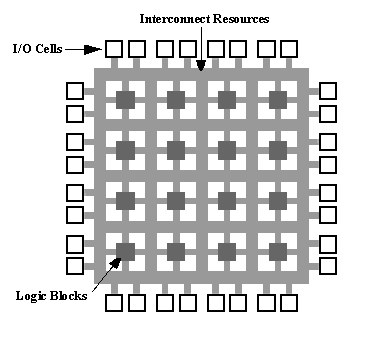
\includegraphics[width=0.5\textwidth,keepaspectratio=true]{./images/fpga1a}
\caption{Componentes de una FPGA}
\label{fig:compfpga}
\end{center}
\end{figure}

	
\subsubsection{Bloques lógicos configurables y lookup tables}

Todas las \textit{FPGAs} se basan en arrays de pequeños elementos de
lógica digital. Los problemas de lógica digital se descomponen en
circuitos lógicos que puedan ser mapeados a una o más de estas
``celdas lógicas'' a través de un proceso llamado \textit{“technology
  mapping"}.
	
Cada bloque de lógica configurable varía de acuerdo a su fabricante,
en el caso de Xilinx tienen el nombre \textit{Logic cell} (LC) (Figura
~\ref{fig:complc}) contiene una LUT de cuatro entradas, un multiplexor
y un registro. Se puede configurar la polaridad del clock, el clock
enable y la señal de reset.

\begin{figure}[h!]
\begin{center}
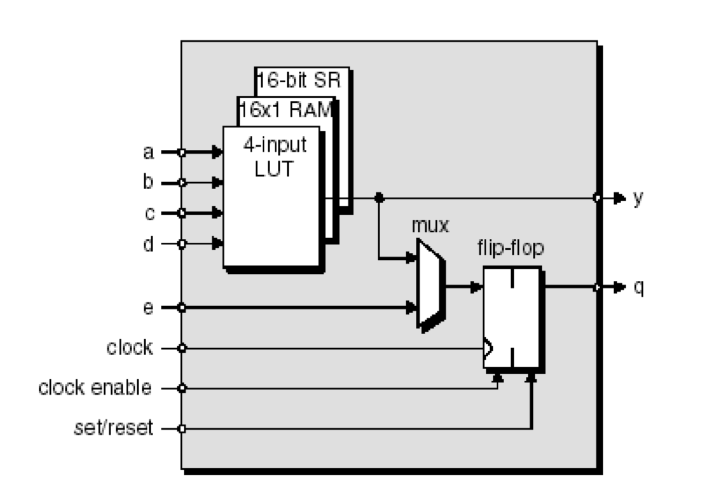
\includegraphics[width=0.5\textwidth,keepaspectratio=true]{./images/celda}
\caption{Componentes de una celda lógica}
\label{fig:complc}
\end{center}
\end{figure}

También se encuentran las \textit{Lookup Tables}, que son elementos
lógicos que están compuestos de al menos un registro programable
(flip\-flop) y alguna lógica de entrada, que usualmente está
implementada como una \textit{lookup table} de n entradas, donde n es
5 o menos. Estas \textit{LUTs} son capaces de implementar cualquier
función combinacional de sus entradas.

\subsubsection{Bloques de entrada y salida de propósito general}

Las \textit{FPGAs} poseen pines TTL, CMOS, PCI, LVDS y muchos otros
que les permiten hacer de interface y convertir tecnologías
diferentes. Las \textit{FPGAs} tienen bloques de I/O dedicados para
clocks y resets globales.
	
También incluyen PLL y esquemas para el manejo de clocks permitiendo
múltiples dominios de los mismos. Las \textit{FPGAs} actuales tienen
impedancias de I/O configurables, permiten el uso de resistencias
internas terminales cuyos valores pueden ser configurados por el
usuario.

\subsubsection{Multiplicadores}

Algunas funciones como los multiplicadores son muy lentos si se
implementan mediante la conexión de un gran numero de bloques
lógicos. Por tal motivo, muchas \textit{FPGAs} incorporan bloques
\textit{multiplicadores} en hardware (Figura ~\ref{fig:mult}). Estos
bloques se encuentran en general muy cerca de los bloques de RAM
embebidos.

\begin{figure}[h!]
\begin{center}
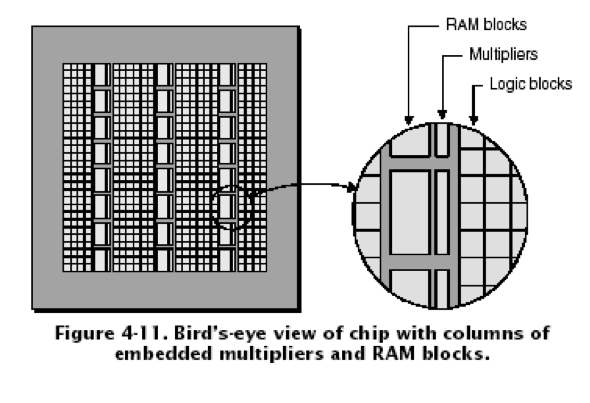
\includegraphics[width=0.5\textwidth,keepaspectratio=true]{./images/multram}
\caption{Multiplicadores}
\label{fig:mult}
\end{center}
\end{figure}

\subsubsection{Manejadores de clock digitales}

El \textit{clock manager} se utiliza para generar un número
determinado de “daughter clocks" (Figura ~\ref{fig:dclocks}). En
particular, es utilizado como \textit{sintetizador de frecuencia} para
remover el \textit{jitter}, donde a partir de una frecuencia de
referencia permite obtener un conjunto discreto de frecuencias. Además
proporciona estabilidad de frecuencia~\cite{Etiqueta03} y
\textit{phase shifting}. Esto último es necesario muchos diseños que
requieren clocks que estén corridos en fase unos con respecto a otros.

\begin{figure}[h!]
\begin{center}
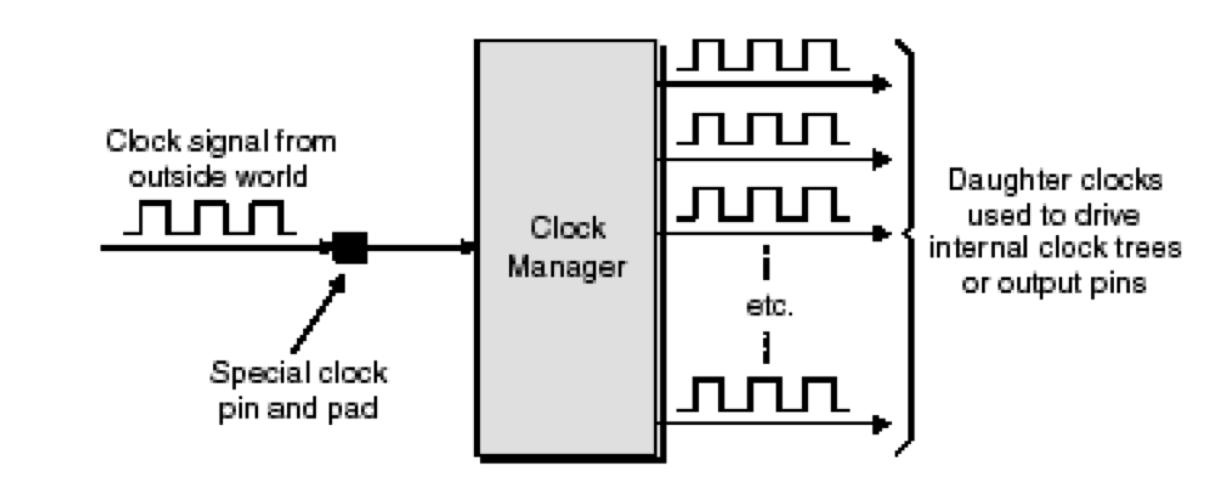
\includegraphics[width=0.5\textwidth,keepaspectratio=true]{./images/dougther}
\caption{Clock manager}
\label{fig:dclocks}
\end{center}
\end{figure}

La FPGA dispone de un \textit{árbol de reloj} (\textit{clock tree})
por el que se distribuye la señal de reloj principal, que es
ramificada para que alcance a todos los flip-flops. Esta estructura
asegura que todos los flip-flop reciban la señal de reloj en forma
síncrona evitando problemas de \textit{skew}. El \textit{árbol de
  reloj} es implementado usando canales independientes a los
utilizados para interconectar los bloques lógicos (Figura
~\ref{fig:ctree}).

\begin{figure}[h!]
\begin{center}
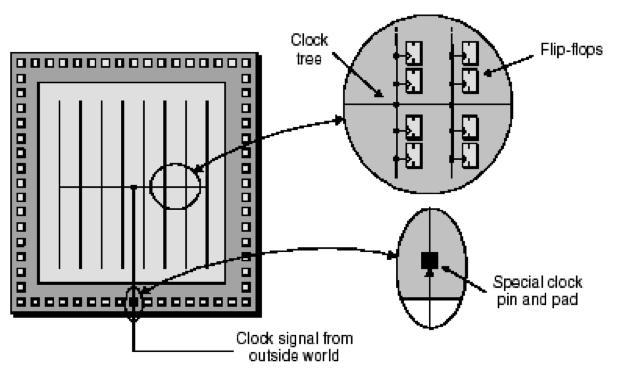
\includegraphics[width=0.5\textwidth,keepaspectratio=true]{./images/clocktree}
\caption{Clock tree}
\label{fig:ctree}
\end{center}
\end{figure}

\subsection{Tipo de tecnología} 

Teniendo en cuenta el tipo de tecnología que utilizan las
\textit{FPGAs} para almacenar sus datos de configuración, estas se
pueden clasificar en tres tipos:

\begin{itemize}
\item \textit {Basadas en memoria RAM estática (SRAM)}: Las
  \textit{FPGAs} guardan su configuración en una memoria interna de
  tipo SRAM. Cada vez que se enciende el sistema es necesario
  reprogramar la \textit{FPGA} con su configuración. Esto hace que sea
  necesario almacenar la configuración en un dispositivo ROM externo o
  descargarla desde un PC conectado a la \textit{FPGA}. Este tipo de
  \textit{FPGA} es la más flexible y permite utilizar técnicas de
  reconfiguración dinámica.
\item \textit{Basadas en memoria ROM}: Las \textit{FPGAs} almacenan su
  configuración en una memoria interna de tipo ROM. Normalmente se
  utiliza una memoria tipo FLASH o EEPROM, siendo la tecnología FLASH
  la dominante en estos momentos. La ventaja se encuentra en que al
  desconectar la energía de la FPGA, la configuración no se pierde y
  por lo tanto no son necesarios componentes externos para
  almacenarla. Como desventaja frente a las FPGA basadas en SRAM, son
  menos flexibles ya que la configuración es más lenta y no permite
  utilizar técnicas de reconfiguración dinámica.
\item \textit{Basadas en fusibles}: La configuración se almacena
  “quemando” fusibles durante el proceso de programación. Actualmente
  la tecnología más utilizada en estas \textit{FPGAs} es la basada en
  anti-fusibles (anti-fuse). La configuración queda grabada en la
  \textit{FPGA} de forma que no es posible reprogramarla, lo que
  elimina cualquier tipo de flexibilidad.
\end{itemize}


\section{IP-Core}
El diseño de circuitos digitales se divide normalmente en bloques
funcionales que se refieren como \textit{módulos} o \textit{cores}. Un
\textit{core} puede influir un conjunto de sub-bloques que ayudan a
poner en práctica su funcionalidad. Los \textit{cores} pueden variar
en tamaño partiendo de la implementación de una simple operación
aritmética hasta la implementación de un microprocesador completo. El
mismo \textit{core} puede ocupar una FPGA entera conformando el
producto final completo o puede ser simplemente un bloque entre otros
en una FPGA más grande o en un ASIC. Los \textit{cores} se describen
generalmente utilizando un lenguaje de descripción de hardware (HDL)
en un nivel de abstracción conocida como Register Transfer Level
(RTL).
	
El proceso de tomar la descripción RTL de un diseño y convertirlo en
un lista de primitivas o puertas lógicas y las conexiones entre ellos,
dejando luego que la implementación se realice en una tecnología de
destino, se conoce como \textit{síntesis}. En forma análoga a la
compilación de software que se tiene un programa en un lenguaje de
alto nivel, como C, y es convertido a codigo maquina; el resultado de
la síntesis, conocido como \textit{netlist}, está en un nivel de
abstracción denominado nivel de la puerta. En pocas palabras, es esta
lista de conexiones la que se utiliza para su posterior procesamiento
en la configuración de una FPGA o en un diseño para ASIC.
	
Los cores pueden ser diseñados por una persona o entidad. Los
desarrolladores de \textit{cores} y licenciatarios varían desde
particulares a empresas. El producto, en este caso se conoce como un
\textit{IP core (Intellectual Property Core)} siendo el diseño la
propiedad intelectual de los desarrolladores.
	
\subsection{Tipos de IP-Cores}

Los \textit{IP cores} se clasifican en:

\begin{itemize}
\item{Softcores} Son los más flexibles y se presentan para \textit{IP}
  en forma netlist (lista de compuertas e interconexiones) o en forma
  de sintetizable RTL, lo que los hace tecnológicamente
  independientes. Los \textit{cores} sintetizable se entregan en un
  lenguaje de descripción de hardware como Verilog o VHDL. Con óptimos
  para ser utilizado en diferentes aplicaciones, pero poseen una menor
  predictibilidad en la implementación y suelen tener un mayor costo y
  menor desempeño de procesamiento.

\item{Firmcores} Los cores firmes están optimizados para ser
  implementados en una FPGA, arquitectura o dispositivo en
  particular. Esta optimización puede ser realizada por el fabricante
  o por un tercero. Utilizar este tipo de IP-Cores requiere disponer
  de cierto nivel de conocimiento de la arquitectura, ya que es
  posible rutear señales físicas y especificar la colocación de los
  elementos de diseño. Un ejemplo de cores firmes es el procesador
  MicroBlaze de Xilinx~\cite{Etiqueta04}

\item{Hardcores} Están optimizados para una tecnología específica y no
  pueden ser modificados por el diseñador que los utiliza. Son
  manifestaciones físicas del diseño del core ya que tienen un layout
  predefinido incluido en la arquitectura. Son los mejores para
  aplicaciones plug\&play. Si bien son poco flexibles, portables y
  configurables, son muy predictibles (el timing es fijo) y fiables
  una vez implementados.
\end{itemize}

\subsection{Microprocesadores softcore reconfigurables}

Como se mencionó en la introducción, el avance en la tecnología de
fabricación VLSI hizo posible la implementación de bloques cada ves
más complejos. Entre estos, los microprocesadores son uno de los
bloques más importantes y de mayor funcionalidad que pueden
implementarse en la actualidad. Originalmente, la implementación de
los mismos estaba limitada a ASIC, pero el avance en las FPGAs hizo
posible la implementación de potentes microprocesadores en las
mismas.

El microprocesador como componente discreto o como parte en un mismo 
chip, es un buen candidato para ser implementado en un FPGA. Esto último introdujo
 un mayor potencial para la exploración
del espacio de diseño en FPGA haciendo que la lógica de cómputo
específica sea implementada junto con un
microprocesador~\cite{Etiqueta05}. En particular, este espacio de
diseño encuentra su máxima riqueza en los microprocesadores softcore
que describiremos a continuación.
	
Dentro de los microprocesadores \textit{Softcore} se encuentra un
grupo que apunta principalmente a la reconfiguración de hardware.
Tres de los más grandes proveedores de FPGA: Xilinx, Altera y Lattice,
ofrecen sus propios núcleos de microprocesadores RISC de 32 bits. Por
otro lado, existes además núcleos \textit{Softcore} \textit{Open
  Source} no limitados por la tecnología. Estos núcleos son
desarrollados en lo general por aficionados en comunidades
\textit{Open Source} o en algunos casos son desarrollados por
entidades comerciales antes de ser \textit{Open Source}.
	
Para los desarrollos dirigidos a una reconfiguración de hardware, la
opción de microprocesadores \textit{Softcore} de 32 bits se encuentra
tanto entre las que opciones que ofrecen los proveedores de FPGA y
como así también esta disponible sin costo en las comunidades
\textit{Open Source}. Sin embargo, existe una importante diferencia a
nivel de licencias entre los productos \textit{Open Source} y los
desarrollados por los proveedores de FPGAs.

Las verdaderas ventajas de \textit{Softcore Open Source} están
relacionadas a la apertura del diseño y la ausencia de restricciones
sobre lo que se puede hacer con el \textit{core}. Con un diseño de
código abierto existe la opción de personalizar la descripción RTL
para implementar la optimización o la funcionalidad deseada. Además,
se logra una mayor la portabilidad y flexibilidad para la
reutilización del producto final.


\subsection{Clasificación de acuerdo con la integración}

El aumento de recursos de las FPGAs junto con la amplia disponibilidad
de bloques IP ha hecho posible la integración de sistemas completos en
la propia FPGA y la aparición de una nueva terminología para
clasificarlos. Algunos de los términos que se usan para clasificar
este tipo de sistemas son:

\begin {itemize}
\item \textit{System on Chip (SoC)}: Circuito integrado formado por
  diversos módulos VLSI con distinta funcionalidad que interconectados
  entre sí ofrecen una funcionalidad específica para una aplicación.
\item \textit{System-on-Programable-Chip (SoPC)}: Se aplica este
  término específicamente cuando el dispositivo utilizado para
  realizar el SoC es reconfigurable.
\item \textit{Configurable-System-on-Chip (CSoC)}: Mediante este
  término se definen los sistemas SoC en los que se hace uso de la
  capacidad de reconfiguración de los mismos para aplicaciones de
  computación reconfigurable. Pueden incluirse bajo la denominación
  CSoC tanto los sistemas que admiten diferentes configuraciones
  estáticas según ciertos condicionantes, como los que utilizan la
  reconfiguración parcial dinámica para modificar en tiempo de
  ejecución una sección hardware.
\item \textit{Multiprocessor-Configurable-System-on-Chip (MCSoC)}: Se
  aplica esta definición a los sistemas CSoC que incluyen varias
  unidades procesador funcionando de forma simultánea.
\end {itemize}

